\documentclass[11pt]{article}
\usepackage{epsfig}
\usepackage{graphicx}
\usepackage{rotating}
\usepackage{amsmath,amsthm}
\usepackage{array}
\usepackage{multirow}
\usepackage{url}
\usepackage{appendix}
\usepackage{algorithm}
\usepackage{algorithmic}
\usepackage{placeins} % FloatBarrier
\usepackage{comment}
\usepackage{enumerate} % Fancy enumeration
\usepackage{appendix}
\usepackage{listings}


\newcommand{\vs}{\vspace{0.1in}}


\usepackage{float}
%\floatstyle{boxed}
%\restylefloat{figure}
\usepackage{morefloats}

\usepackage{caption}


\lstset{breaklines=true}


\oddsidemargin=0in
\evensidemargin=0in
\textwidth=6.5in
%\textwidth=6.42in (if no footnote)
\textheight=8.75in
%\textheight=9.1in (if no footnote)
%\topmargin=-0.5cm
%\topmargin=0.5in
\footskip=1.0cm
\headheight=0pt
%\newcommand{\comment}[1]{}

\setlength{\extrarowheight}{5pt}

\theoremstyle{definition}
\newtheorem{definition}{Definition}
\newtheorem*{examples}{Examples}
\newtheorem{example}{}

\begin{document}

\title{An Empirical Evaluation of Denoising\\Techniques for Streaming Data}

\date{\today}

%

\author{Jeremy Luke Thompson\thanks{United States Air Force Academy and Lawrence Livermore National Laboratory}}


%\vfill
%\vspace{2.0in}
\maketitle


\begin{abstract}
In this paper, we focus on denoising techniques for streaming data that are analyzed while being collected. We investigate spatial filters, such as the Box filter, Gaussian smoothing, and the Bilateral filter, frequency techniques, such as Fourier transform coefficient thresholding and wavelet transform coefficient thresholding, and a statistical neighborhood filter, Non-Local Means. These methods are applied to both synthetic data and real world data. We discuss practical concerns for incremental implementation, such as edge treatment, incremental updating, and parameter stability. We note situations when these methods fail and make recommendations for use with real world data, specifically for the use of one or two iterations of the same Bilateral filter or a combination of the Bilateral and Non-Local Means filters.
\end{abstract}

%\thispagestyle{empty} %\vspace{2.0in}

%\vfill \eject


%\thispagestyle{empty}

%\clearpage

\pagestyle{plain}
\pagenumbering{arabic}


%%%%%%%%%%%%%%%%%%%%%%%%%%%%%%%%%%%%%%%%%%%%%%%%%%%%%%%%%%%%%%%%%%%%%%%%%%


 
\section{Time Series Data and Noise}

A time series is any temporally ordered series of observations. Frequently, as when collecting observations of various real world phenomenon, these observations will be contaminated with a variety of errors, or noise, such as sampling and processing errors. In this paper, we consider various techniques for denoising time series data received incrementally. We discuss multiple classes of techniques and practical considerations for incremental implementation such as edge treatment, incremental updating, and parameter selection. Additionally, we assess the performance of these techniques in the context of peak signal to noise ratio for known time series with added noise and optimal parameter stability.

Many deniosing techniques rely upon an estimate of the variance of the distribution this random noise comes from, typically assumed to be Gaussian. Gasser, et al.~\cite{Gasser86} describes a method for estimating this unknown value based upon the sum of squared differences between the observed data and linear interpolations approximating the true values of the time series. In this paper, we use the notation $y_i$ for the values of the time series at time index $i$. For a time series with $N$ values, starting at $i = 0$, the estimated noise variance is:

\begin{displaymath}
\hat{\sigma} ^2_n = \frac{2}{3 \left( N - 2 \right)} \sum _{i = 1} ^{N - 2} \left( \frac{1}{2} y_{i - 1} - y_i + \frac{1}{2} y_{i + 1} \right) ^2
\end{displaymath}

We use this estimate to set the parameters of some of the denoising techniques we investigate. There are, naturally, a variety of other techniques for noise variance estimation, with different levels of robustness and computational difficultly. This technique is used here because of its simplicity.

The remainder of this paper is organized in three parts, a description of the denoising techniques we will use in Section 2, an empirical evaluation of the effect of the parameters when denoising know time series in Section 3, and conclusions and recommendations with suggestions for future work in Section 4.


\section{Denoising Techniques}

There are a variety of denosing techniques, and they fit into three broad categories, local smoothing filters, frequency coefficient thresholding techniques, and statistical neighborhood filters. We discuss three spatial filters, the box filter, Gaussian filter, and Bilateral filter, two frequency techniques, Fourier transform coefficient thresholding and wavelet transform coefficient thresholding, and one statistical neighborhood filter, Non-Local Means.

\vs
\noindent
\textbf{Box Filter:} The box filter is the simplest denoising technique and is a uniformly weighted moving average of the time series. This technique works best in time series with true values that do not change rapidly so the noise averages to zero over an interval while the true time series values remain relatively unchanged. Smoothed values are given by

\begin{displaymath}
s_i = \sum _{j \in I} w \left(i, j \right) y_j
\end{displaymath}

\noindent
where the weights are given by the function

\begin{displaymath}
w\left(i, j\right) = \frac{1}{\lvert I \rvert}
\end{displaymath}

\noindent
and $\lvert I \rvert$ is the size of the interval, or window, of the filter. Typically the interval is symmetric about the point of interest, which means $\lvert I \rvert$ is odd. In this technique, the interval size is a parameter to be chosen by the analyst. Figure \ref{boxdemo} shows the weighting scheme for the box filter.

The color convention for charts in this paper is black for the true time series values, if known, blue for the noisy time series values, red for the denoised time series values, and cyan for the residuals, the difference between the noisy and denoised time series values.

\begin{figure}
\centering
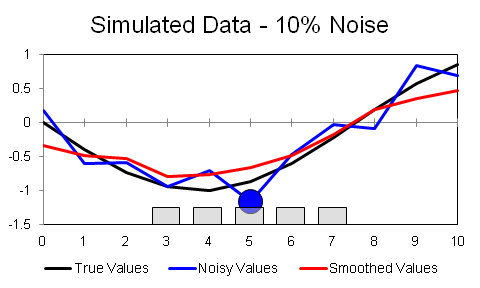
\includegraphics[width = 0.65 \textwidth]{BoxDemo.png}
\caption{Box Filter Weighting Scheme}
\label{boxdemo}
\end{figure}

In time series where intensity values change rapidly, this technique removes features of interest in the time series. Figure \ref{boxcompare} shows the performance of the box filter on simulated data generated from the composition of two sine functions and a sawtooth function. The box filter does a reasonable job removing noise, but it destroys features in the time series, such as the three jumps at the end of these sawteeth. The damage to the three jumps can be seen in the residuals, show in cyan in the figure. This damage is one of the reasons the box filter is not used in practice.

\begin{figure}
\centering
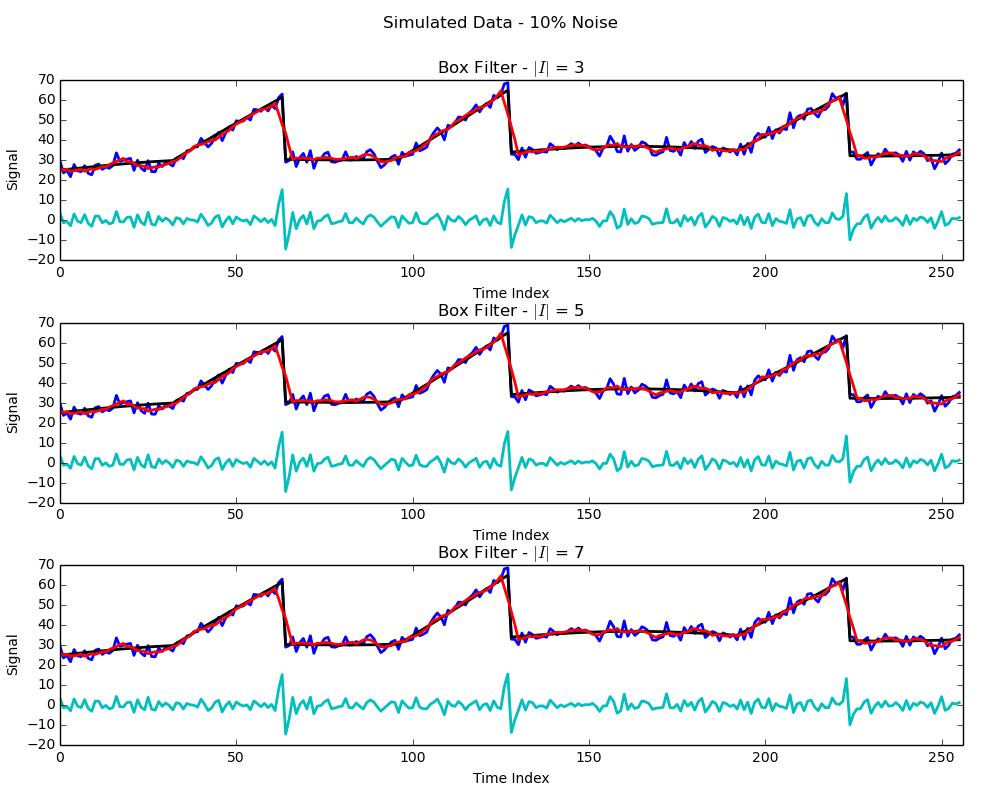
\includegraphics[width = 0.65 \textwidth]{BoxCompare.png}
\caption{Box Filter With Simulated Data}
\label{boxcompare}
\end{figure}

It is important to note that treatment of edge values is particularly important when incrementally processing a time series as the most relevant data is in the leading edge of the data set. In the case of spatial filters, the $\frac{\lvert I \rvert - 1}{2}$ values on each edge do not have complete intervals. We adjust normalization factor $z_i$ to ensure that the weight values in the incomplete interval still sum to $1$. Figure \ref{increment} shows the adjusted weighting scheme for the box filter for the most recent data point, highlighted in blue.

With this edge treatment, it is simple to adjust the time series when a new data point is received. With the updated time series, the last $\frac{\lvert I \rvert - 1}{2}$ smoothed values can be updated and a new smoothed value can be calculated as before. Figure \ref{increment} also highlights the updated values, in red. This comments on edge treatment and incrementing also apply to our implementation of the other spatial filters, namely the Gaussian and Bilateral filters.

\begin{figure}
\centering
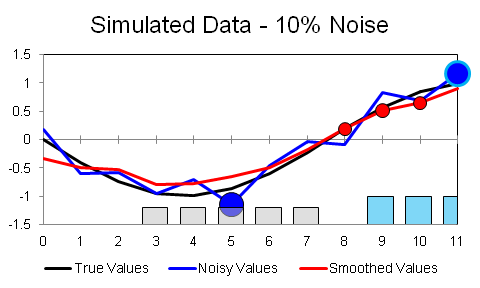
\includegraphics[width = 0.65 \textwidth]{Increment.png}
\caption{Updated Edge Values for Local Smoothing Filters}
\label{increment}
\end{figure}

\vs
\noindent
\textbf{Gaussian Filter:} The Gaussian filter is a weighted moving average that weights points based upon their distance from the point of interest according to a Gaussian distribution with standard deviation $\sigma_d$. The smoothed values from the Gaussian filter are given by

\begin{displaymath}
s_i = \sum _{j \in I} w \left(i, j \right) y_j
\end{displaymath}

\noindent
where the weights are given by the function

\begin{displaymath}
w\left(i, j\right) = \frac{1}{z_i} e^{-\frac{\lvert i - j \rvert}{2 \sigma_d^2}}
\end{displaymath}

\noindent
and $z_i$ is a normalization factor so the weights sum to $1$ on the interval.

Typically a interval width of $10 \sigma_d$ is used. This accounts for $99.99994\%$ of the Gaussian distribution. Some computations can be saved by using an interval width of $8 \sigma_d$, $99.994\%$ of the Gaussian distribution, or $6 \sigma_d$, $99.7\%$ of the Gaussian distribution. In this technique, the Gaussian kernel standard deviation, $\sigma_d$, is a parameter to be chosen by the analyst. Figure \ref{gaussiandemo} shows the weighting scheme for the Gaussian filter.

\begin{figure}
\centering
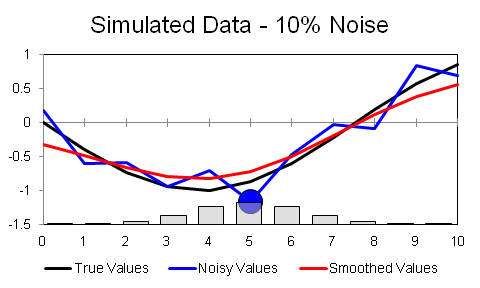
\includegraphics[width = 0.65 \textwidth]{GaussianDemo.png}
\caption{Gaussian Filter Weighting Scheme}
\label{gaussiandemo}
\end{figure}

As seen in Figure \ref{gaussiancompare}, the Gaussian filter does a reasonable job removing noise but also destroys features in the time series, albeit to a lesser degree than for a box filter with the same window size. The damage to the three jumps can again be seen in the residuals, show in cyan in the figure.

\begin{figure}
\centering
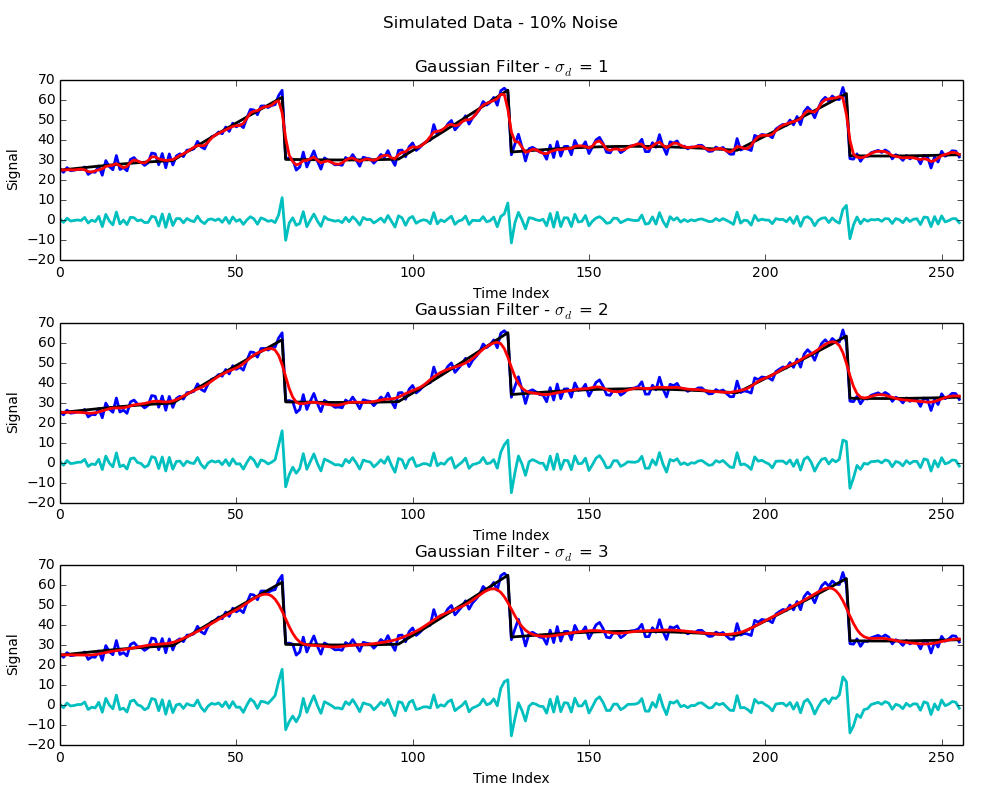
\includegraphics[width = 0.65 \textwidth]{GaussianCompare.png}
\caption{Gaussian Filter with Simulated Data}
\label{gaussiancompare}
\end{figure}

\vs
\noindent
\textbf{Bilateral Filter:} The Bilateral filter attempts to better preserve features in the time series by applying a pair of Gaussian weights, one for spatial distance, as in the Gaussian filter, and one for differences in intensity values. The smoothed values from the Bilateral filter are given by

\begin{displaymath}
s_i = \sum _{j \in I} w \left(i, j \right) y_j
\end{displaymath}

\noindent
where the weights are given by the function

\begin{displaymath}
w\left(i, j\right) = \frac{1}{z_i} e^{-\frac{\lvert i - j \rvert}{2 \sigma_d^2}}e^{-\frac{\lvert y_i - y_j \rvert}{2 \sigma_i^2}}
\end{displaymath}

\noindent
and, as before, $z_i$ is a normalization factor.

As before, an interval width of $10 \sigma$ is typical. In this technique, the Gaussian kernel standard deviations, $\sigma_d$ and $\sigma_i$, are two parameters to be chosen by the analyst. Figure \ref{bilateraldemo} shows the weighting scheme for the Bilateral filter.

\begin{figure}
\centering
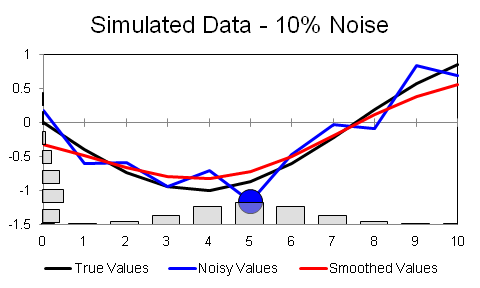
\includegraphics[width = 0.65 \textwidth]{BilateralDemo.png}
\caption{Bilateral Filter Weighting Scheme}
\label{bilateraldemo}
\end{figure}

As seen in Figure \ref{bilateralcompare}, the bilateral filter does a reasonable job both smoothing the time series and retaining features. Damage to the three jumps cannot be seen in the residuals. Unfortunately, the Bilateral filter may retain some of the noise, particularly if the noise causes a significant change in intensity value.

\begin{figure}
\centering
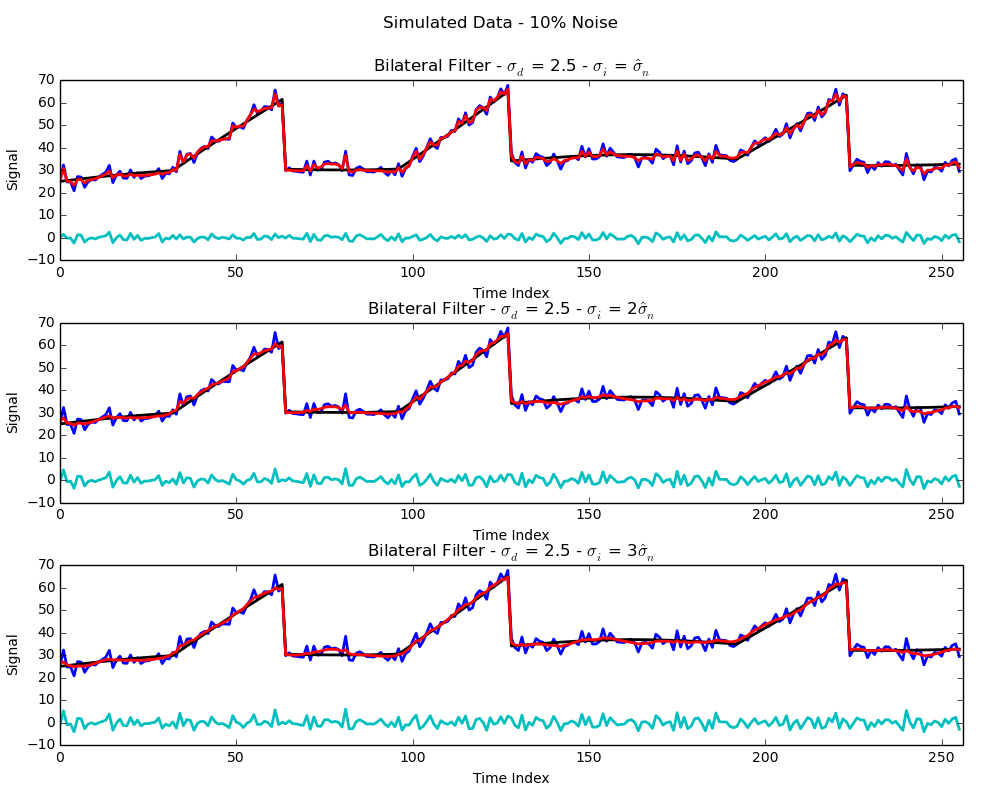
\includegraphics[width = 0.65 \textwidth]{BilateralCompare.png}
\caption{Bilateral Filter with Simulated Data}
\label{bilateralcompare}
\end{figure}

Zang and Gunturk~\cite{Zang08} suggest that the optimal value of the standard deviation of the spatial Gaussian kernel, $\sigma_d$, is in the range $\left[ 1.5, 2.1 \right]$ and the standard deviation of the intensity Gaussian kernel, $\sigma_i$, is in the range $\left[ 1.5 \sigma_n, 3 \sigma_n \right]$ for $2$D image processing. It is uncertain if these results translate to $1$D time series denoising.

\vs
\noindent
\textbf{Fourier Transform:} Historically, analysis in the frequency domain was conducted via the Fourier transform in its rapid discrete form, the Fast Fourier Transform (FFT). The FFT takes uniformly spaced observations and can transform the data relatively quickly. After transformation, coefficient thresholding is used on the time series frequency coefficients to denoise the data, and then the denoised frequency coefficients are reverse transformed.

There are two common procedures for modifying noisy frequency coefficients, known as thresholding methods~\cite{Donoho94}. The first, hard thresholding, cancels all coefficients smaller than a particular threshold. $v\left(\alpha\right)$ represents the frequency coefficients of the time series, the result of transforming data. In hard thresholding, the denoised coefficients are given by:

\begin{displaymath}
v\left(\alpha\right) = 
\begin{cases}
v\left(\alpha\right) & \lvert v\left(\alpha\right)\rvert > \mu \\
0 & \lvert v\left(\alpha\right)\rvert < \mu
\end{cases}
\end{displaymath}

Hard thresholding can create wavelet outliers, which can be partially avoided using soft thresholding. In soft thresholding the denoised coefficients are given by:

\begin{displaymath}
v\left(\alpha\right) = 
\begin{cases}
v\left(\alpha\right) - sgn\left(v\left(\alpha\right)\right)\mu & \lvert v\left(\alpha\right)\rvert \geq \mu \\
0 & \lvert v\left(\alpha\right)\rvert < \mu
\end{cases}
\end{displaymath}

Unfortunately, soft thresholding can create problems with the scale of the reverse transformed data which can make it inappropriate for time series were the scale of the data is important. For this reason, we will only consider hard thresholding. In this algorithm, the analyst can control the choice of hard or soft thresholding and the thresholding cutoff, $\mu$.

The theoretically optimal threshold is $\mu = \sigma \sqrt{2 log I}$, where $I$ is the number of data points and $\sigma$ is the standard deviation of the coefficients. In order to avoid inflating the standard deviation of the coefficients through a large coefficient corresponding to the mean of the data, the mean is subtracted from the time series prior to transformation, making the time series a zero-mean dataset. In practice this threshold is too high and cancels too many coefficients that do not correspond to noise. Instead, $\mu = 3 \sigma$ is used for hard thresholding and $\mu = \frac{3}{2} \sigma$ is used for soft thresholding~\cite{Buades05} for $2$D image processing. It is uncertain if these results translate to $1$D time series denoising.

As can be seen in Figure \ref{fftcompare}, the Fourier transform struggles near the edges, where Gibbs phenomenon may occur. This makes the Fourier transform less than ideal for incremental data denoising, where the most relevant data is near the end of the time series.

\begin{figure}
\centering
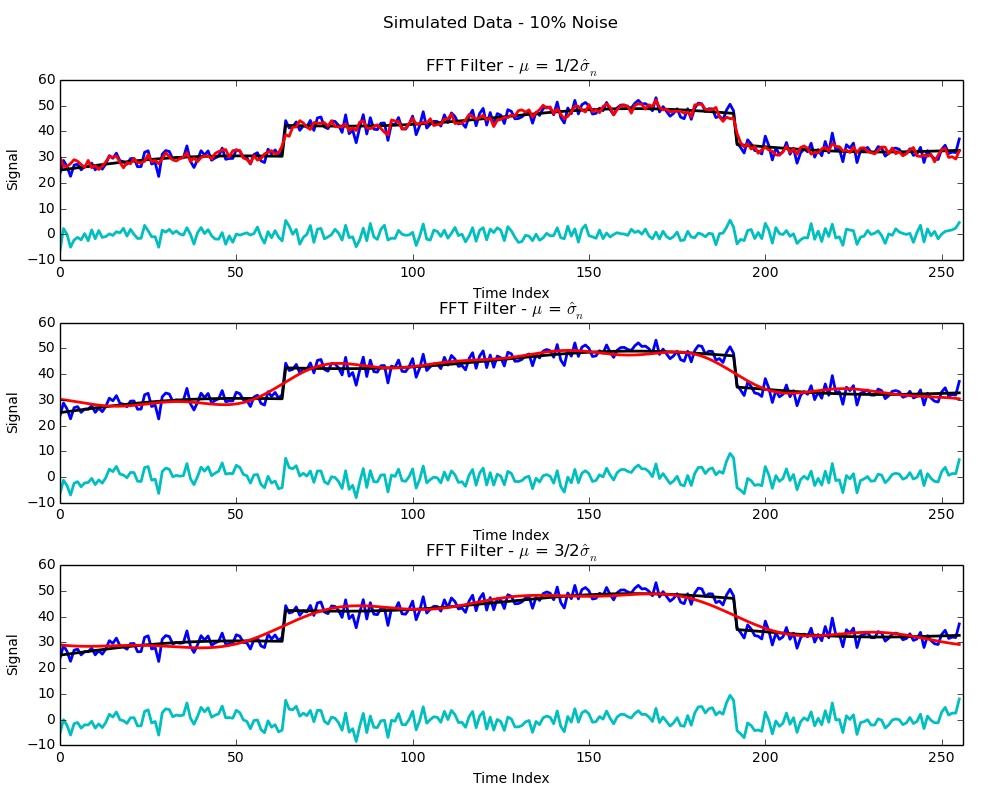
\includegraphics[width = 0.65 \textwidth]{FFTCompare.png}
\caption{Fourier Transform Filter with Simulated Data}
\label{fftcompare}
\end{figure}

Incremental updates present a problem for the Fourier transform, as the transform can only be applied to multiple data points, and the larger the number the better. This means that it takes more computations to incrementally update Fourier transform coeficient thresholding smoothed time series than locally smoothed time series.

\vs
\noindent
\textbf{Wavelet Transform:} The wavelet transform is one of the most popular frequency domain alternatives to the Fourier transform. While the Fourier transform completely transforms the time series into the frequency domain, the wavelet transform offers both frequency and time information by fitting a series of finite length functions, wavelets, to the time series. One such wavelet is the Harr wavelet, Figure \ref{harrwavelet}. This allows for filtering both by frequency and temporal relationships~\cite{Graps95}. There are a variety of wavelet families to choose from, and the wavelet transformations can be repeated to a desired level of resolution. We use the Harr wavelet due to its simplicity, but many other families of wavelets give better performance.

\begin{figure}
\centering
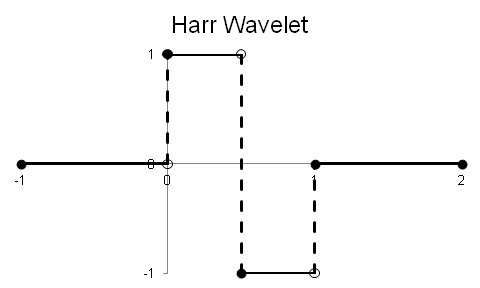
\includegraphics[width = 0.65 \textwidth]{HarrWavelet.png}
\caption{Harr Wavelet}
\label{harrwavelet}
\end{figure}

Mota, Vasconcelos, and Silva~\cite{Mota05} outlined a algorithm for processing continuous data streams in real time using the discrete wavelet transform, inspired by an older result by Vishwanath, called the Recursive Pyramid Algorithm~\cite{Vishwanath94}.

Once the data has been wavelet transformed, the data is denoised via frequency coefficient thresholding, as with the Fourier transform.

In this technique, the analyst choses the wavelet family, the number of levels of decomposition, and the thresholding cutoff, $\mu$. Figure \ref{waveletcompare} shows the results from denoising with a Harr wavelet transform, with different hard thresholds.

\begin{figure}
\centering
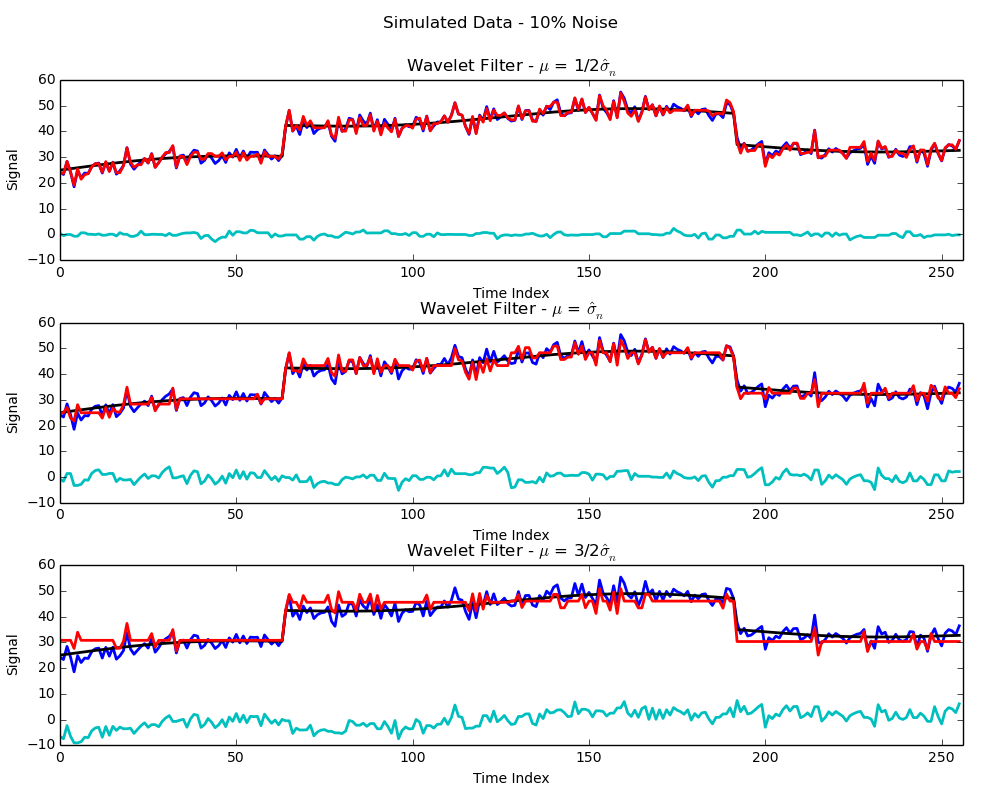
\includegraphics[width = 0.65 \textwidth]{WaveletCompare.png}
\caption{Wavelet Transform Filter with simulated data}
\label{waveletcompare}
\end{figure}

In this case, there is no special edge treatment. Incremental data processing is often accomplished via a real time algorithm, as mentioned above and frequency coefficients are thresholded and back transformed immediately afterwards.

\vs
\noindent
\textbf{Non-Local Means:} Statistical neighborhood filters attempt to fix the problems associated with local smoothing filters by calculating the smoothed value as a weighted average of other values in the time series based upon the similarity between the neighborhoods around the time series values. Figure \ref{nlmeansdemo} shows three neighborhoods highlighted in the time series. The values in the green window are more similar to the values in the black window than the values in the red window and, thus, should be weighted higher.

The Non-Local Means algorithm was first introduced by Buades et al.~\cite{Buades05}. Non-Local Means has primarily been used for image processing, but it has been mentioned in a $1$D context in several papers (~\cite{Galiano13}, ~\cite{Tracey12}, ~\cite{Zoican10}). We use a modification of this algorithm for efficient $3$D medical image processing by Coup{\'e} et al.~\cite{Coupe07}.

\begin{figure}
\centering
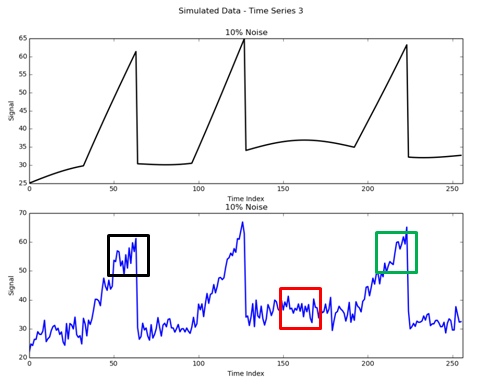
\includegraphics[width = 0.65 \textwidth]{NLMeansDemo.png}
\caption{Non-Local Means Window Comparison}
\label{nlmeansdemo}
\end{figure}

In the Non-Local Means algorithm, smoothed values are given by

\begin{displaymath}
s_i = \sum _{j \in N} w \left(i, j \right) y_j
\end{displaymath}

\noindent
where the weights are given by the function

\begin{displaymath}
w \left(i, j \right) = \frac{1}{z_i} e^{-\frac{\lvert Y_i - Y_j \rvert ^2}{2 \beta \hat{\sigma}^2_n \lvert Y \rvert}}
\end{displaymath}

In this scheme, $Y_i$ is a vector of intensity values in the window, or neighborhood, around $y_i$, $\lvert Y_i - Y_j \rvert$ is the $L_2$ norm of the difference in intensity values in these intervals, $\lvert Y \rvert$ is the window size, and $\beta$ is a parameter chosen by the analyst to control the amount of smoothing. According to Coup{\'e} et al.~\cite{Coupe07}, $\beta$ varies between $0.0$ and $1.0$, with values of $\beta$ closer to $1.0$ better for high levels of noise and values of $\beta$ closer to $0.5$ better for lower levels of noise.

Duval et al.~\cite{Duval11} notes that neighborhood preselection can improve the results of the Non-Local Means algorithm by assigning a weight of $0$ to the $y_j$ values that have neighborhoods that are too dissimilar to the neighborhood, $Y_i$, under consideration. Duval et al. uses a preslection test based upon the norm of the difference between neighborhoods. A more complex preselection method is described by Buades et al.~\cite{Buades05}. We use Duval et al.'s preselection test:

\begin{displaymath}
w\left(i, j\right) = 
\begin{cases}
\frac{1}{z_i} e^{-\frac{\lvert Y_i - Y_j \rvert ^2}{2 \beta \hat{\sigma}^2_n \lvert Y \rvert}} & \lvert Y_i - Y_j \rvert < T \\
0 & $otherwise$
\end{cases}
\end{displaymath}

Duval et al.~\cite{Duval11} suggests that values of $T$ near $20$ or $30$ work well for $2$D images. This threshold does make sense for denosing time series. We will consider thresholds of the type $T = \delta \left( \mathrm{max} Y_j - \mathrm{min} Y_j \right) \lvert Y \rvert$, where $\delta \in \left[ 0.0, 1.0 \right]$. This threshold is a percentage of an approximation of the maximum intensity interval distance. Duval et al. recommends window sizes of $5$ or $7$ for $2$D image processing. As before, it is uncertain if these results translate to $1$D time series denoising.

In this algorithm, the analyst can control the amount of smoothing via $\beta$, the preselection parameter $\delta$, the window size, and the portion of the time series that is compared. Figure \ref{nlmeanscompare} shows the performance of the Non-Local Means technique with different values of $\beta$. Notice how similar the performance is to the Bilateral filter, Figure \ref{bilateralcompare}.

\begin{figure}
\centering
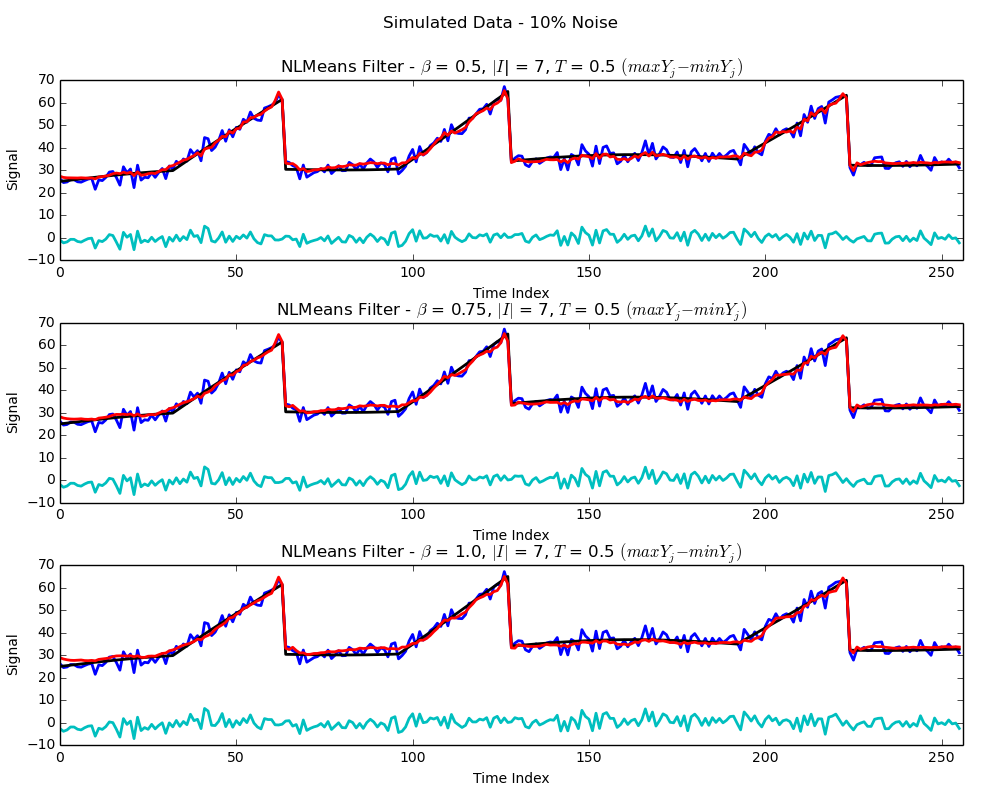
\includegraphics[width = 0.65 \textwidth]{NLMeansCompare.png}
\caption{Non-Local Means Filter with Simulated Data}
\label{nlmeanscompare}
\end{figure}

As with the spatial filters, the $\frac{\lvert I \rvert - 1}{2}$ values on the edges do not have complete intervals, or windows. In order to calculate weights, we compare the incomplete neighborhood $Y_i$ with incomplete neighborhoods around the other points $Y_j$. We adjust normalization factor $z_i$ to ensure that the weight values in the incomplete interval still sum to $1$.

With this edge treatment, it is simple to adjust the time series when a new data point is received. With the updated time series, the last $\frac{\lvert I \rvert - 1}{2}$ smoothed values can be updated and a new smoothed value can be calculated as before.

\vs
\noindent
\textbf{Combination Techniques:} There are a variety of ways to combine or iterate these techniques.

Iterating the box filter and Gaussian filter is well understood and is equivalent to using a box filter or Gaussian filter with a wider interval or larger kernel, $\sigma_d$. We do not investigate these here. Iterating the Fourier transform or wavelet transform coefficient thresholding is equivalent to using a Fourier transform or wavelet transform filter with a higher frequency coefficient threshold. We do will not investigate these here either. We also do not consider combinations of frequency and spatial or statistical neighborhood techniques.

Iterating a Bilateral filter or Non-Local Means filter is more complex. Also, the question of combining a Bilateral filter and Non-Local Means filter is open. We will investigate all three of these possibilities.


\section{Comparison}

In this section we the results of the denoising techniques for time series. We will consider both known time series with added noise and real world time series. First, we consider optimal choices for the standpoint of peak signal to noise ratio (PSNR) for known time series with added noise. Then, we view the effect of these parameters on real world data.


\subsection{Known Time Series} PSNR, peak signal to noise ratio, is a measure of how noisy a signal is, and therefore how effective a denoising algorithm was. It is calculated as follows:

\begin{displaymath}
PSNR = 10 \mathrm{log} _{10} \left( \frac{\mathrm{max} _{i \in \Omega} ^2 \left( y_i \right)}{MSE} \right)
\end{displaymath}

where $MSE$, mean square error, is

\begin{displaymath}
MSE = \frac{1}{N} \sum _{i = 0} ^{N - 1} \left( y_i - s_i \right) ^2
\end{displaymath}

It is important to note that PSNR is one of the most popular, but not the only, measure of quality for a denoised time series. PSNR is a global measure of quality, where higher values indicate a less noisy signal. An ideal denoising method is relatively insensitive to parameter choice within an optimal range and provides the best increase in PSNR.

One of the most popular noise models is Additive White Gaussian Noise (AWGN). AWGN is comprised of independent identically distributed real values from the Gaussian distribution with known, or more commonly unknown, standard deviation, $\sigma_n$. 

We are assessing the performance of the denoising techniques with three known time series, shown in Figure \ref{signalscompare} with $10$\% noise added, with $1$, $5$, $10$, $20$, and $30$ percent AWGN noise added. Noise of a particular percentage is added by using $\sigma_n = v p$ as the standard deviation of the distribution that generated the noise, were $v$ is the maximum possible range of values that the time series could take and $p$ is the percentage.

\begin{figure}
\centering
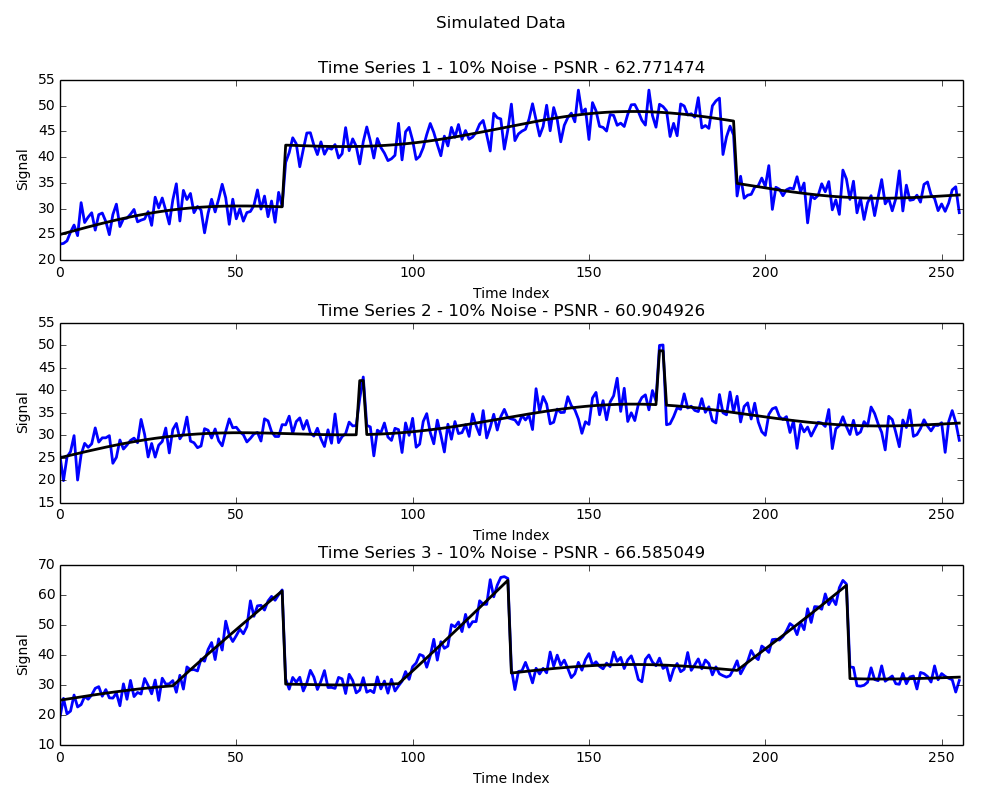
\includegraphics[width = 0.65 \textwidth]{SignalsCompare.png}
\caption{Known Time Series - 10\% Noise}
\label{signalscompare}
\end{figure}

All of the time series were created by taking low frequency sinusoidal behavior and adding features of interest. There are a few interesting observations that can be made about the three time series.

The first time series was created by taking low frequency sinusoidal behavior and adding a sharp increase in intensity one quarter of the way through the time series and adding a sharp decrease in intensity three quarters of the way through the time series. In some cases the noise obscures the sharp increase or decrease in intensity, making it appear to be a more gradual increase or decrease in intensity. Noise can make features impossible to recover.

The second time series was created by taking low frequency sinusoidal behavior and adding two brief, sharp increases in intensity, at one and two thirds of the way through the time series. In some cases the noise can become indistinguishable from these features, making them impossible to recover.

The third time series was created by taking low frequency sinusoidal behavior and adding three sawtooth features, at one, three, and six eights of the way through the time series. As with the first time series, it is possible for the noise to obscure the sharp decrease at the end of the saw tooth features, making it appear to be a more gradual decrease in intensity.

The average PSNR values for the time series without denoising are shown in Figure \ref{noisypsnr}. An ideal result offers significantly higher PSNR values and is relatively insensitive to small changes in parameter choice.

\begin{table}
\small
\begin{center}
\begin{tabular}{l | c | c | c}
 & Time Series 1 & Time Series 2 & Time Series 3 \\ \hline
1\% Noise & 85.546 & 72.155 & 67.335 \\ \hline
5\% Noise & 81.121 & 70.323 & 66.857 \\ \hline
10\% Noise & 73.582 & 66.015 & 65.038 \\ \hline
20\% Noise & 63.132 & 57.815 & 60.987 \\ \hline
30\% Noise & 56.497 & 51.587 & 56.220
\end{tabular}
\caption{Noisy PSNR}
\label{noisypsnr}
\end{center}
\end{table}

These denoising techniques were first assessed in a full factorial design over the following parameter ranges:

\begin{enumerate}

\item Noise: $1$\%, $5$\%, $10$\%, $20$\%, and $30$\%

\item $\lvert I \rvert$: $3$, $5$, $7$, and $9$

\item $\sigma_d$: $0.1$, $1.0$, $2.0$, $3.0$, and $4.0$

\item $\sigma_i$: $0.1 \hat{\sigma}_n$, $1.0 \hat{\sigma}_n$, $2.0 \hat{\sigma}_n$, $3.0 \hat{\sigma}_n$, and $4.0 \hat{\sigma}_n$

\item $\mu$: $0.1 \sigma$, $1.0 \sigma$, $2.0 \sigma$, and $3.0 \sigma$

\item $\beta$: $0.5$, $0.75$, and $1.0$

\item $\lvert Y \rvert$: $3$, $5$, $7$, and $9$

\item $\delta$: $0.25$, $0.5$, and $0.75$

\end{enumerate}

$5$ iterations were run at each combination of parameters for each denoising method. Further iterations were run for finer resolution at parameter values that appeared to be near optimal for each denoising method, increasing the resolution of the grid in areas of interest. For each iteration, a new noisy signal was created, denoised, and then PSNR was calculated.

\vs
\noindent
\textbf{Box Filter:} The box filter is not used in practice, but results are included here as a comparison point.

Table \ref{boxbestpsnr} shows the best performance of the box filter in the search area. Table \ref{boxselectpsnr} shows the performance of the box filter when $\lvert I \rvert = 7$. The PSNR value for this parameter setting and the percentage of the maximum PSNR value are listed in each cell. The box filter consistently produces poor performance, but the performance is stable across the values of the parameter in the search area.

\begin{table}[!h]
\small
\begin{center}
\begin{tabular}{l | c | c | c}
 & Time Series 1 & Time Series 2 & Time Series 3 \\ \hline
1\% Noise & 85.594 & 72.175 & 67.346 \\ \hline
5\% Noise & 81.206 & 70.377 & 66.771 \\ \hline
10\% Noise & 74.047 & 66.201 & 65.354 \\ \hline
20\% Noise & 64.323 & 58.005 & 60.920 \\ \hline
30\% Noise & 56.888 & 52.199 & 57.145
\end{tabular}
\caption{Box Filter Best PSNR}
\label{boxbestpsnr}
\end{center}
\end{table}

\begin{table}[!h]
\small
\begin{center}
\begin{tabular}{l | c | c | c}
 & Time Series 1 & Time Series 2 & Time Series 3 \\ \hline
1\% Noise & 85.549/99.9\% & 72.175/100.0\% & 67.346/100.0\% \\ \hline
5\% Noise & 81.059/99.8\% & 70.181/99.7\% & 66.747/100.0\% \\ \hline
10\% Noise & 73.249/98.9\% & 66.040/99.8\% & 64.923/99.3\% \\ \hline
20\% Noise & 62.786/97.6\% & 57.932/99.9\% & 60.631/99.5\% \\ \hline
30\% Noise & 56.165/98.7\% & 51.829/99.3\% & 56.082/98.1\%
\end{tabular}
\caption{Box Filter Selected Parameter PSNR - $\lvert I \rvert = 7$}
\label{boxselectpsnr}
\end{center}
\end{table}

\vs
\noindent
\textbf{Gaussian Filter:} The Gaussian filter does not perform significantly better than the box filter.

Table \ref{gaussianbestpsnr} shows the best performance of the Gaussian filter in the search area. Table \ref{gaussianselectpsnr} shows the performance of the Gaussian filter when $\sigma_d = 2.25$. The PSNR value for this parameter setting and the percentage of the maximum PSNR value are listed in each cell. The Gaussian filter also consistently produces poor performance, but the performance is stable across the values of the parameter in the search area. The performance is slightly better than the box filter and slightly less stable.

\begin{table}[!h]
\small
\begin{center}
\begin{tabular}{l | c | c | c}
 & Time Series 1 & Time Series 2 & Time Series 3 \\ \hline
1\% Noise & 83.257 & 71.659 & 74.807 \\ \hline
5\% Noise & 80.684 & 70.459 & 79.871 \\ \hline
10\% Noise & 75.844 & 68.646 & 69.177 \\ \hline
20\% Noise & 69.529 & 60.971 & 62.031 \\ \hline
30\% Noise & 61.243 & 56.495 & 58.172
\end{tabular}
\caption{Gaussian Filter Best PSNR}
\label{gaussianbestpsnr}
\end{center}
\end{table}

\begin{table}[!h]
\small
\begin{center}
\begin{tabular}{l | c | c | c}
 & Time Series 1 & Time Series 2 & Time Series 3 \\ \hline
1\% Noise & 83.257/100.0\% & 71.659/100.0\% & 63.953/85.5\% \\ \hline
5\% Noise & 80.684/100.0\% & 70.459/100.0\% & 63.685/79.7\% \\ \hline
10\% Noise & 75.844/100.0\% & 67.568/98.4\% & 62.980/91.0\% \\ \hline
20\% Noise & 67.086/96.5\% & 60.005/98.4\% & 60.437/97.4\% \\ \hline
30\% Noise & 59.973/97.9\% & 54.554/96.6\% & 56.797/97.6\%
\end{tabular}
\caption{Gaussian Filter Selected Parameter PSNR - $\sigma_d = 2.25$}
\label{gaussianselectpsnr}
\end{center}
\end{table}

\vs
\noindent
\textbf{Bilateral Filter:} The Bilateral filter offers significantly improved performance compared to both the box and Gaussian filters.

Table \ref{bilateralbestpsnr} shows the best performance of the Bilateral filter in the search area. Table \ref{bilateralselectpsnr} shows the performance of the Bilateral filter when $\sigma_d = 2.5$ and $\sigma_i = 2.5 \hat{\sigma}_n$. The PSNR value for this parameter setting and the percentage of the maximum PSNR value are listed in each cell. The Bilateral filter performs well and is reasonably stable in the search area. The performance is significantly better than the box or Gaussian filters and slightly less stable.

\begin{table}[!h]
\small
\begin{center}
\begin{tabular}{l | c | c | c}
 & Time Series 1 & Time Series 2 & Time Series 3 \\ \hline
1\% Noise & 127.251 & 128.396 & 121.790 \\ \hline
5\% Noise & 97.303 & 96.758 & 96.698 \\ \hline
10\% Noise & 81.774 & 78.128 & 84.987 \\ \hline
20\% Noise & 69.794 & 63.453 & 70.033 \\ \hline
30\% Noise & 62.657 & 59.049 & 61.736
\end{tabular}
\caption{Bilateral Filter Best PSNR}
\label{bilateralbestpsnr}
\end{center}
\end{table}

\begin{table}[!h]
\small
\begin{center}
\begin{tabular}{l | c | c | c}
1\% Noise & 124.947/98.2\% & 126.752/98.7\% & 110.432/90.7\% \\ \hline
5\% Noise & 93.220/95.8\% & 92.841/96.0\% & 96.698/100.0\% \\ \hline
10\% Noise & 79.580/97.3\% & 75.578/96.7\% & 84.480/99.4\% \\ \hline
20\% Noise & 64.659/92.6\% & 60.585/95.5\% & 68.456/97.7\% \\ \hline
30\% Noise & 57.875/92.4\% & 53.774/91.1\% & 60.891/98.6\%
\end{tabular}
\caption{Bilateral Filter Selected Parameters PSNR - $\sigma_d = 2.5$, $\sigma_i = 2.5 \hat{\sigma}_n$}
\label{bilateralselectpsnr}
\end{center}
\end{table}

\vs
\noindent
\textbf{Fourier Transform:} Fourier transform coefficient thresholding does not appear to be as effective as the Bilateral filter, giving performance equivalent to the box and Gaussian filters.

Table \ref{fftbestpsnr} shows the best performance of Fourier transform coefficient thresholding in the search area. Table \ref{fftselectpsnr} shows the performance of Fourier transform coefficient thresholding when $\mu = 0.15 \sigma$. The PSNR value for this parameter setting and the percentage of the maximum PSNR value are listed in each cell. Fourier transform coefficient thresholding particularly struggles with a fixed thresholding level, which is likely why methods such as SURE~\cite{Rangarajan02} are so popular with frequency based techniques. Fourier transform coefficient thresholding also has significantly less stable optimal parameters compared to the local neighborhood techniques.

\begin{table}[!h]
\small
\begin{center}
\begin{tabular}{l | c | c | c}
 & Time Series 1 & Time Series 2 & Time Series 3 \\ \hline
1\% Noise & 75.495 & 64.912 & 72.728 \\ \hline
5\% Noise & 74.657 & 65.029 & 71.950 \\ \hline
10\% Noise & 69.444 & 61.559 & 66.948 \\ \hline
20\% Noise & 63.094 & 57.928 & 58.394 \\ \hline
30\% Noise & 59.586 & 57.348 & 51.886
\end{tabular}
\caption{Fourier Transform Coefficient Thresholding Best PSNR}
\label{fftbestpsnr}
\end{center}
\end{table}

\begin{table}[!h]
\small
\begin{center}
\begin{tabular}{l | c | c | c}
 & Time Series 1 & Time Series 2 & Time Series 3 \\ \hline
1\% Noise & 70.638/93.6\% & 62.517/96.3\% & 67.359/92.6\% \\ \hline
5\% Noise & 70.752/94.8\% & 62.200/95.6\% & 66.589/92.5\% \\ \hline
10\% Noise & 69.444/100.0\% & 61.559/100.0\% & 65.227/97.4\% \\ \hline
20\% Noise & 53.774/85.2\% & 49.052/84.7\% & 55.580/95.2\% \\ \hline
30\% Noise & 45.173/75.8\% & 41.630/72.6\% & 48.409/93.3\%
\end{tabular}
\caption{Fourier Transform Coefficient Thresholding Selected Parameter PSNR - $\mu = 0.15 \sigma$}
\label{fftselectpsnr}
\end{center}
\end{table}

\vs
\noindent
\textbf{Wavelet Transform:} Wavelet transform coefficient thresholding also gives performance similar to the box and Gaussian filters.

Table \ref{waveletbestpsnr} shows the best performance of wavelet transform coefficient thresholding in the search area. Table \ref{waveletselectpsnr} shows the performance of wavelet transform coefficient thresholding when $\mu = 0.3 \sigma$. The PSNR value for this parameter setting and the percentage of the maximum PSNR value are listed in each cell. Wavelet transform coefficient thresholding also struggles with a fixed thresholding level and also struggles high levels of noise. At low levels of noise wavelet transformation coefficient thresholding is almost as effective as the Bilateral filter. Wavelet transform coefficient thresholding also has significantly less stable optimal parameters compared to the local neighborhood techniques.

\begin{table}[!h]
\small
\begin{center}
\begin{tabular}{l | c | c | c}
 & Time Series 1 & Time Series 2 & Time Series 3 \\ \hline
1\% Noise & 104.704 & 105.849 & 103.423 \\ \hline
5\% Noise & 76.321 & 74.722 & 80.334 \\ \hline
10\% Noise & 64.351 & 61.333 & 67.268 \\ \hline
20\% Noise & 51.839 & 49.754 & 54.477 \\ \hline
30\% Noise & 46.453 & 51.175 & 47.660
\end{tabular}
\caption{Wavelet Transform Coefficient Thresholding Best PSNR}
\label{waveletbestpsnr}
\end{center}
\end{table}

\begin{table}[!h]
\small
\begin{center}
\begin{tabular}{l | c | c | c}
 & Time Series 1 & Time Series 2 & Time Series 3 \\ \hline
1\% Noise & 87.042/83.1\% & 86.556/81.8\% & 91.880/88.8\% \\ \hline
5\% Noise & 76.321/100.0\% & 73.853/98.8\% & 79.821/99.4\% \\ \hline
10\% Noise & 63.265/98.3\% & 61.333/100.0\% & 67.268/100.0\% \\ \hline
20\% Noise & 50.248/96.9\% & 46.852/94.2\% & 52.868/97.0\% \\ \hline
30\% Noise & 44.178/95.1\% & 40.057/78.3\% & 47.362/99.4\%
\end{tabular}
\caption{Wavelet Transform Coefficient Thresholding Selected Parameter PSNR - $\mu = 0.3 \sigma$}
\label{waveletselectpsnr}
\end{center}
\end{table}

\vs
\noindent
\textbf{Non-Local Means:} Non-Local Means ofers performance that is nearly equivalent to the Bilateral filter.

Table \ref{nlmeansbestpsnr} shows the best performance of the Bilateral filter in the search area. Table \ref{nlmeansselectpsnr} shows the performance of the Bilateral filter when $\beta = 0.5$, $\lvert I \rvert = 7$, and $T = 0.75 \left( \mathrm{max} Y_j - \mathrm{min} Y_j \right)$. The PSNR value for this parameter setting and the percentage of the maximum PSNR value are listed in each cell. The Non-Local Means filter has similar, but slightly inferior performance to the Bilateral filter.

It is worth noting that the optimal value for the parameter $\beta$ did increase as the noise level of the time series increased. It is an open question if $\beta$ could be set with a fixed relationship between the variance of the time series and the estimated noise variance.

Theoretically, Non-Local Means should work better on longer time series. An area of future research would be to consider this stability analysis on significantly longer time series. It is known that the computation time is much longer and the preselection is much more significant for Non-Local Means on large time series.

\begin{table}[!h]
\small
\begin{center}
\begin{tabular}{l | c | c | c}
 & Time Series 1 & Time Series 2 & Time Series 3 \\ \hline
1\% Noise & 114.852 & 112.238 & 101.050 \\ \hline
5\% Noise & 89.317 & 89.332 & 92.007 \\ \hline
10\% Noise & 77.760 & 75.828 & 79.996 \\ \hline
20\% Noise & 65.997 & 60.698 & 68.439 \\ \hline
30\% Noise & 58.928 & 54.630 & 62.217
\end{tabular}
\caption{Non-Local Means Filter Best PSNR}
\label{nlmeansbestpsnr}
\end{center}
\end{table}

\begin{table}[!h]
\small
\begin{center}
\begin{tabular}{l | c | c | c}
 & Time Series 1 & Time Series 2 & Time Series 3 \\ \hline
1\% Noise & 114.852/98.0\% & 112.238/98.1\% & 101.050/98.0\% \\ \hline
5\% Noise & 89.317/98.6\% & 89.332/97.4\% & 92.007/98.1\% \\ \hline
10\% Noise & 77.760/95.7\% & 75.828/95.1\% & 79.996/98.8\% \\ \hline
20\% Noise & 65.997/95.5\% & 60.698/95.0\% & 68.439/96.6\% \\ \hline
30\% Noise & 58.928/96.5\% & 54.630/99.6\% & 62.217/96.1\%
\end{tabular}
\caption{Non-Local Means Filter Selected Parameters PSNR - $\beta = 0.5$, $\lvert I \rvert = 7$, $\delta = 0.75$}
\label{nlmeansselectpsnr}
\end{center}
\end{table}

\vs
\noindent
\textbf{Combination Techniques:}

We consider several combination techniques: two different iterations of the Bilateral filter, two iterations of the same Bilateral filter, iterating the Bilateral filter until the result changes by less than 1\%, two different iterations of Non-Local Means, and a combination of the Bilateral filter and Non-Local Means.

\vs
\textbf{2 Different Bilateral Filters:} Two different iterations of the Bilateral filter offered slightly improved performance compared to a single iteration of the Bilateral filter.

Table \ref{2diffbilateralbestpsnr} shows the best performance of two different iterations of the Bilateral filter in the search area. Table \ref{2diffbilateralselectpsnr} shows the performance of two different iterations of the Bilateral filter when $\sigma_{d1} = 2.5$, $\sigma_{i1} = 2.0 \hat{\sigma}_n$, $\sigma_{d2} = 3.0$, and $\sigma_{i2} = 2.5 \hat{\sigma}_n$. The PSNR value for this parameter setting and the percentage of the maximum PSNR value are listed in each cell. Two different iterations of the Bilateral filter performs well and is reasonably stable in the search area. The performance is slightly better than a single iteration of the Bilateral filter and also slightly less stable.

\begin{table}[!h]
\small
\begin{center}
\begin{tabular}{l | c | c | c}
 & Time Series 1 & Time Series 2 & Time Series 3 \\ \hline
1\% Noise & 128.702 & 129.586 & 106.938 \\ \hline
5\% Noise & 102.541 & 101.245 & 97.853 \\ \hline
10\% Noise & 87.505 & 84.902 & 88.481 \\ \hline
20\% Noise & 72.558 & 67.433 & 74.769 \\ \hline
30\% Noise & 65.472 & 60.479 & 65.889
\end{tabular}
\caption{2 Different Bilateral Filters Best PSNR}
\label{2diffbilateralbestpsnr}
\end{center}
\end{table}

\begin{table}[!h]
\small
\begin{center}
\begin{tabular}{l | c | c | c}
 & Time Series 1 & Time Series 2 & Time Series 3 \\ \hline
1\% Noise & 124.219/96.5\% & 124.732/96.3\% & 98.953/92.5\% \\ \hline
5\% Noise & 97.096/94.7\% & 97.972/96.8\% & 92.550/94.6\% \\ \hline
10\% Noise & 83.758/95.7\% & 78.568/92.5\% & 84.086/95.0\% \\ \hline
20\% Noise & 68.950/95.0\% & 62.641/92.9\% & 72.100/96.4\% \\ \hline
30\% Noise & 62.052/94.8\% & 58.350/96.5\% & 65.094/98.8\%
\end{tabular}
\caption{2 Different Bilateral Filters Selected Parameters PSNR -}
 $\sigma_{d1} = 2.5$, $\sigma_{i1} = 2.0 \hat{\sigma}_n$, $\sigma_{d2} = 3.0$, $\sigma_{i2} = 2.5 \hat{\sigma}_n$
\label{2diffbilateralselectpsnr}
\end{center}
\end{table}

\vs
\textbf{2 Same Bilateral Filters:} Two iterations of the same Bilateral filter offered slightly improved performance compared to a single iteration of the Bilateral filter.

Table \ref{2samebilateralbestpsnr} shows the best performance of two iterations of the same Bilateral filter in the search area. Table \ref{2samebilateralselectpsnr} shows the performance of two iterations of the same Bilateral filter when $\sigma_{d1} = 2.5$, $\sigma_{i1} = 2.0 \hat{\sigma}_n$, $\sigma_{d2} = 3.0$, and $\sigma_{i2} = 2.5 \hat{\sigma}_n$. The PSNR value for this parameter setting and the percentage of the maximum PSNR value are listed in each cell. Two iterations of the same Bilateral filter performs well and is reasonably stable in the search area. The performance is comparable to two different iteration of the Bilateral filter.

\begin{table}[!h]
\small
\begin{center}
\begin{tabular}{l | c | c | c}
 & Time Series 1 & Time Series 2 & Time Series 3 \\ \hline
1\% Noise & 126.790 & 128.683 & 108.250 \\ \hline
5\% Noise & 103.260 & 101.220 & 99.692 \\ \hline
10\% Noise & 87.270 & 84.463 & 88.091 \\ \hline
20\% Noise & 71.926 & 66.703 & 73.766 \\ \hline
30\% Noise & 65.420 & 57.585 & 64.878
\end{tabular}
\caption{2 Same Bilateral Filters Best PSNR}
\label{2samebilateralbestpsnr}
\end{center}
\end{table}

\begin{table}[!h]
\small
\begin{center}
\begin{tabular}{l | c | c | c}
 & Time Series 1 & Time Series 2 & Time Series 3 \\ \hline
1\% Noise & 124.104/97.9\% & 125.701/97.7\% & 97.981/90.5\% \\ \hline
5\% Noise & 98.423/95.3\% & 98.219/97.0\% & 91.889/92.2\% \\ \hline
10\% Noise & 83.413/95.6\% & 80.776/95.6\% & 84.786/96.2\% \\ \hline
20\% Noise & 69.228/96.2\% & 65.098/97.6\% & 71.679/97.2\% \\ \hline
30\% Noise & 61.121/93.4\% & 57.585/100.0\% & 64.878/100.0\%
\end{tabular}
\caption{2 Same Bilateral Filters Selected Parameters PSNR - $\sigma_d = 3.0$, $\sigma_i = 2.0 \hat{\sigma}_n$}
\label{2samebilateralselectpsnr}
\end{center}
\end{table}

\vs
\textbf{Bilateral Filter Iterated to Tolerance:} Multiple iterations of the same Bilateral filter offered performance comparable to a single iteration of the Bilateral filter.

Table \ref{itrbilateralbestpsnr} shows the best performance of multiple iterations of the same Bilateral filter in the search area. Table \ref{itrbilateralselectpsnr} shows the performance of multiple iterations of the same Bilateral filter when $\sigma_d = 3.0$, and $\sigma_i = 2.5 \hat{\sigma}_n$. The PSNR value for this parameter setting and the percentage of the maximum PSNR value are listed in each cell. Two iterations of the same Bilateral filter performs well and is reasonably stable in the search area. The performance can be lower than a single iteration of the Bilateral filter. The stability of the optimal parameters is lower than for a single iteration of the Bilateral filter.

\begin{table}[!h]
\small
\begin{center}
\begin{tabular}{l | c | c | c}
 & Time Series 1 & Time Series 2 & Time Series 3 \\ \hline
1\% Noise & 126.387 & 128.682 & 120.867 \\ \hline
5\% Noise & 100.102 & 102.022 & 98.848 \\ \hline
10\% Noise & 86.418 & 85.543 & 87.412 \\ \hline
20\% Noise & 72.479 & 67.397 & 73.564 \\ \hline
30\% Noise & 63.684 & 60.820 & 65.202
\end{tabular}
\caption{Iterated Bilateral Filter Best PSNR}
\label{itrbilateralbestpsnr}
\end{center}
\end{table}

\begin{table}[!h]
\small
\begin{center}
\begin{tabular}{l | c | c | c}
 & Time Series 1 & Time Series 2 & Time Series 3 \\ \hline
1\% Noise & 123.012/97.3\% & 126.306/98.2\% & 96.433/79.8\% \\ \hline
5\% Noise & 99.427/99.3\% & 97.578/95.6\% & 93.087/94.2\% \\ \hline
10\% Noise & 84.112/97.3\% & 74.561/87.2\% & 84.502/96.7\% \\ \hline
20\% Noise & 69.483/95.9\% & 64.130/95.2\% & 73.112/99.4\% \\ \hline
30\% Noise & 62.807/98.6\% & 53.906/88.6\% & 63.868/98.0\%
\end{tabular}
\caption{Iterated Bilateral Filter Selected Parameters PSNR - $\sigma_d = 3.0$, $\sigma_i = 2.5 \hat{\sigma}_n$}
\label{itrbilateralselectpsnr}
\end{center}
\end{table}

\vs
\textbf{2 Different Non-Local Means Filters:} Two iterations of Non-Local Means offered slightly worse performance compared to a single iteration of Non-Local Means.

Table \ref{2diffnlmeansbestpsnr} shows the best performance of two iterations of Non-Local Means in the search area. Table \ref{2diffnlmeansselectpsnr} shows the performance of two iterations of Non-Local Means when $\beta_1 = 0.3333$, $\lvert Y \rvert _1 = 7$, $\delta _1 = 0.6666$, $\beta_2 = 0.3333$, $\lvert Y \rvert _2 = 7$, and $\delta _2 = 0.3333$. The PSNR value for this parameter setting and the percentage of the maximum PSNR value are listed in each cell. Two iterations of Non-Local Means does not perform as well as a single iteration but is reasonably stable in the search area.

\begin{table}[!h]
\small
\begin{center}
\begin{tabular}{l | c | c | c}
 & Time Series 1 & Time Series 2 & Time Series 3 \\ \hline
1\% Noise & 107.847 & 104.524 & 91.865 \\ \hline
5\% Noise & 89.297 & 90.918 & 89.758 \\ \hline
10\% Noise & 77.988 & 76.564 & 81.663 \\ \hline
20\% Noise & 67.315 & 64.974 & 69.230 \\ \hline
30\% Noise & 60.147 & 59.249 & 62.978
\end{tabular}
\caption{2 Different Non-Local Means Best PSNR}
\label{2diffnlmeansbestpsnr}
\end{center}
\end{table}

\begin{table}[!h]
\small
\begin{center}
\begin{tabular}{l | c | c | c}
 & Time Series 1 & Time Series 2 & Time Series 3 \\ \hline
1\% Noise & 107.847/100.0\% & 102.152/97.7\% & 90.914/99.0\% \\ \hline
5\% Noise & 87.114/97.6\% & 87.728/96.5\% & 86.901/96.8\% \\ \hline
10\% Noise & 76.152/97.6\% & 75.499/98.6\% & 80.257/98.3\% \\ \hline
20\% Noise & 62.439/92.8\% & 60.393/92.9\% & 66.626/96.2\% \\ \hline
30\% Noise & 59.260/98.5\% & 55.082/93.0\% & 60.762/96.5\%
\end{tabular}
\caption{2 Different Non-Local Means Selected Parameters PSNR -}
 $\beta_1 = 0.3333$, $\lvert Y \rvert _1 = 7$, $\delta _1 = 0.6666$, $\beta_2 = 0.3333$, $\lvert Y \rvert _2 = 7$, $\delta _2 = 0.3333$
\label{2diffnlmeansselectpsnr}
\end{center}
\end{table}

\vs
\textbf{Bilateral and Non-Local Means Combination:} The combination of Bilateral and Non-Local Means filters offered improved performance compared to either method alone.

Table \ref{bilateralnlmeansbestpsnr} shows the best performance of the combination of Bilateral and Non-Local Means in the search area. Table \ref{bilateralnlmeansselectpsnr} shows the performance of the combination of Bilateral and Non-Local Means when $\sigma_d = 2.5$, $\sigma_i = 1.8 \hat{\sigma}_n$, $\beta = 0.5$, $\lvert Y \rvert = 7$, and $\delta = 0.9$. The PSNR value for this parameter setting and the percentage of the maximum PSNR value are listed in each cell. The combination of Bilateral and Non-Local Means performs well and is reasonably stable in the search area.

\begin{table}[!h]
\small
\begin{center}
\begin{tabular}{l | c | c | c}
 & Time Series 1 & Time Series 2 & Time Series 3 \\ \hline
1\% Noise & 116.272 & 114.415 & 110.231 \\ \hline
5\% Noise & 100.498 & 97.932 & 97.620 \\ \hline
10\% Noise & 87.153 & 82.641 & 86.879 \\ \hline
20\% Noise & 73.244 & 66.868 & 75.505 \\ \hline
30\% Noise & 67.219 & 60.023 & 84.472
\end{tabular}
\caption{Bilateral and Non-Local Means Filters Best PSNR}
\label{bilateralnlmeansbestpsnr}
\end{center}
\end{table}

\begin{table}[!h]
\small
\begin{center}
\begin{tabular}{l | c | c | c}
 & Time Series 1 & Time Series 2 & Time Series 3 \\ \hline
1\% Noise & 114.572/98.5\% & 111.731/97.7\% & 94.137/85.4\% \\ \hline
5\% Noise & 94.730/94.3\% & 94.948/97.0\% & 89.549/91.7\% \\ \hline
10\% Noise & 79.659/91.4\% & 78.388/94.9\% & 77.953/89.7\% \\ \hline
20\% Noise & 66.427/90.7\% & 61.955/92.7\% & 66.799/88.5\% \\ \hline
30\% Noise & 60.274/89.7\% & 57.825/96.3\% & 84.472/100.0\%
\end{tabular}
\caption{Bilateral and Non-Local Means Filters Selected Parameters PSNR -}
$\sigma_d = 2.5$, $\sigma_i = 1.8 \hat{\sigma}_n$, $\beta = 0.5$, $\lvert Y \rvert = 7$, $\delta = 0.9$
\label{bilateralnlmeansselectpsnr}
\end{center}
\end{table}

\vs
\noindent
\textbf{Comparison for 10\% Noise:} Figure \ref{comparisonbest} shows a comparison of the best performance of each method for all three time series at 10\% noise, and Figure \ref{comparisonselected} shows a comparison of the selected parameter performance between all methods considered for all three time series at 10\% noise.

Some trends can be seen from these charts. The box filter, Gaussian filter, Fourier transform coefficient thresholding, and wavelet transform coefficient thresholding consistently offer the worst performance, and all of these methods may in fact reduce PSNR for the time series. Of the remaining techniques, multiple iterations of the Bilateral filter to tolerance has very inconsistent performance, sometime performing well and other times being the worst of the remaining techniques.

Two iterations of Non-Local Means often has worse performance than a single iteration, and two different iterations of the Bilateral filter also often has worse performance than a single iteration. The consistent top performers are the Bilateral filter and two iterations of the same Bilateral Filter. These techniques offered a 15\% to 30\% improvement with the selected parameters.

Figures \ref{timeseries1simulatedcompare}, \ref{timeseries2simulatedcompare}, and \ref{timeseries3simulatedcompare} show the performance of the methods without the combinations on the known time series with $10$\% noise added.

The spike at time index $85$ in time series 2 is a good example of a feature that is sufficiently obscured by noise to make it almost impossible to fully recover. The increase in intensity at time index $64$ in time series 1 provides an example of the intensity of the jump being decreased due to positive noise values on the lower side of the jump and negative noise values on the upper side of the jump.

As expected, the box and Gaussian filters destroy features in these time series while the Bilateral filter or Non-Local Means appear to do well at denoising the time series while retaining features. This can be seen particularly well with the jumps in time series 1, the spikes in time series 2, and the sawteeth in time series 3.

Fourier transform and wavelet transform coefficient thresholding appear to denoise less than either the Bilateral filter or Non-Local Means in all three time series.

\begin{table}
\small
\begin{center}
\begin{tabular}{l | c | c | c}
 & Time Series 1 & Time Series 2 & Time Series 3 \\ \hline
Noisy & 73.582 & 66.015 & 65.038 \\ \hline
Box Filter & 74.047 & 66.201 & 65.354 \\ \hline
Gaussian Filter & 75.844 & 68.646 & 69.177 \\ \hline
Bilateral Filter & 81.774 & 78.128 & 84.987 \\ \hline
Fourier Transform & 69.444 & 61.559 & 66.948 \\ \hline
Wavelet Transform & 64.351 & 61.333 & 67.268 \\ \hline
Non-Local Means & 77.760 & 75.828 & 79.996 \\ \hline
2 Different Bilateral & 87.505 & 84.902 & 88.481 \\ \hline
2 Same Bilateral & 87.270 & 84.463 & 88.091 \\ \hline
Iterated Bilateral & 86.418 & 85.543 & 87.412 \\ \hline
2 Different NL Means & 77.988 & 76.564 & 81.663 \\ \hline
Bilateral NL Means & 87.153 & 82.641 & 86.879
\end{tabular}
\caption{Performance Comparison at 10\% Noise - Best Performance}
\label{comparisonbest}
\end{center}
\end{table}

\begin{table}
\small
\begin{center}
\begin{tabular}{l | c | c | c}
 & Time Series 1 & Time Series 2 & Time Series 3 \\ \hline
Noisy & 73.582 & 66.015 & 65.038 \\ \hline
Box Filter &73.249/98.9\% &66.040/99.8\% & 64.923/99.3\% \\ \hline
Gaussian Filter & 75.844/100.0\% & 67.568/98.4\% & 62.980/91.0\% \\ \hline
Bilateral Filter & 79.580/97.3\% & 75.578/96.7\% & 84.480/99.4\% \\ \hline
Fourier Transform & 69.444/100.0\% & 61.559/100.0\% & 65.227/97.4\% \\ \hline
Wavelet Transform & 63.265/98.3\% & 61.333/100.0\% & 67.268/100.0\% \\ \hline
Non-Local Means & 77.760/95.7\% & 75.828/95.1\% & 79.996/98.8\% \\ \hline
2 Different Bilateral & 83.758/95.7\% & 78.568/92.5\% & 84.086/95.0\% \\ \hline
2 Same Bilateral & 83.413/95.6\% & 80.776/95.6\% & 84.786/96.2\% \\ \hline
Iterated Bilateral & 84.112/97.3\% & 74.561/87.2\% & 84.502/96.7\% \\ \hline
2 Different NL Means & 76.152/97.6\% & 75.499/98.6\% & 80.257/98.3\% \\ \hline
Bilateral NL Means & 79.659/91.4\% & 78.388/94.9\% & 77.953/89.7\%
\end{tabular}
\caption{Performance Comparison at 10\% Noise - Selected Parameters}
\label{comparisonselected}
\end{center}
\end{table}

\begin{figure}[h!]
\centering
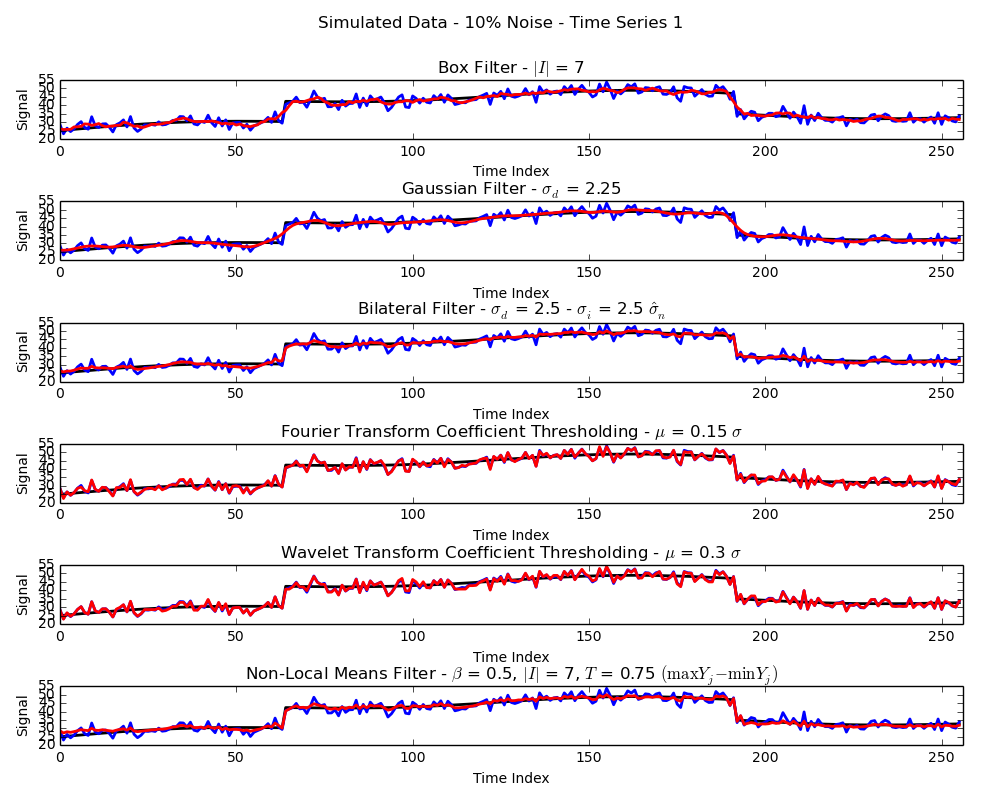
\includegraphics[width = 0.95 \textwidth]{TimeSeries1SimulatedCompare.png}
\caption{Comparison on Simulated Data - Time Series 1}
\label{timeseries1simulatedcompare}
\end{figure}

\begin{figure}[h!]
\centering
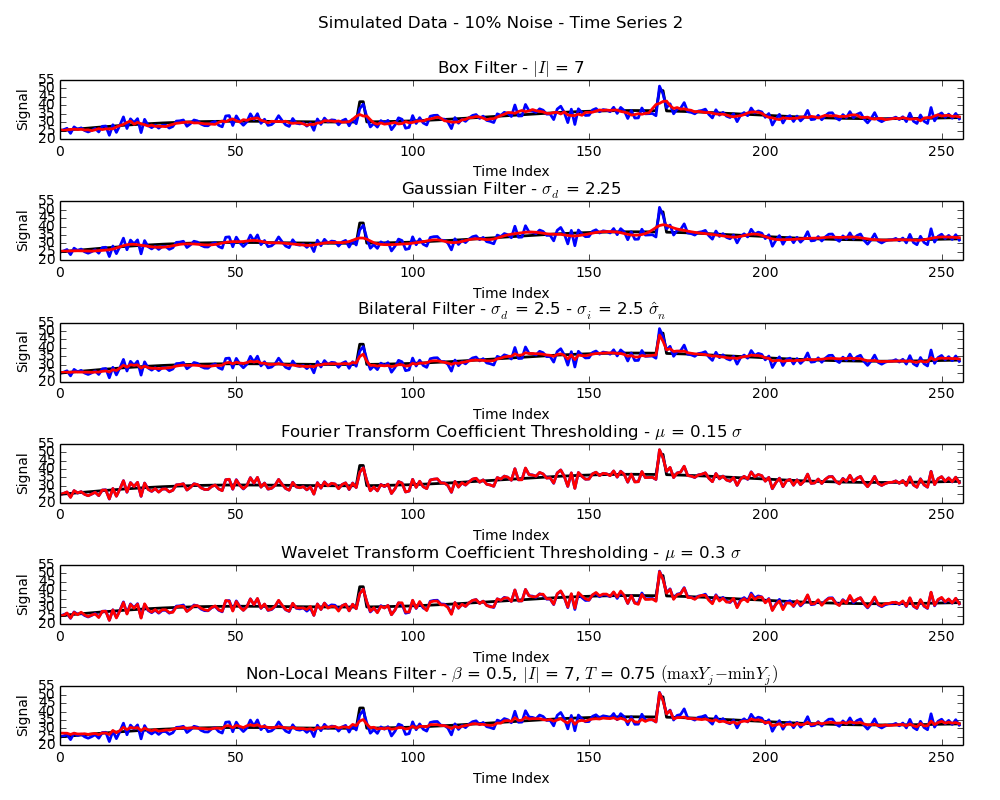
\includegraphics[width = 0.95 \textwidth]{TimeSeries2SimulatedCompare.png}
\caption{Comparison on Simulated Data - Time Series 2}
\label{timeseries2simulatedcompare}
\end{figure}

\begin{figure}[h!]
\centering
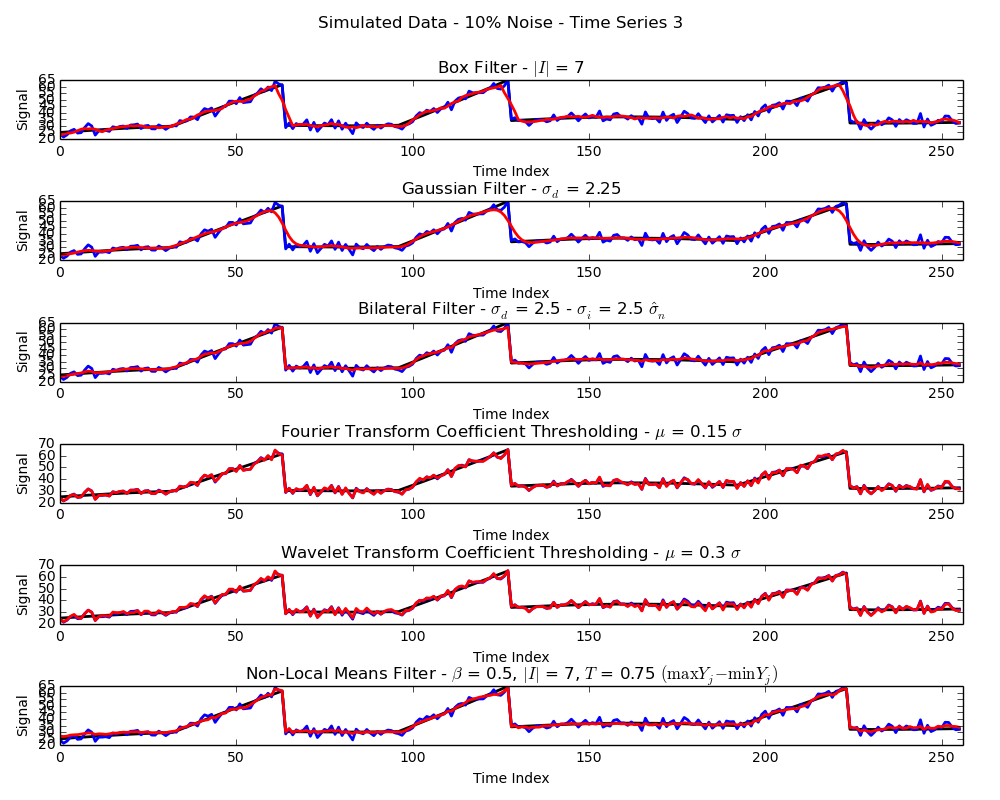
\includegraphics[width = 0.95 \textwidth]{TimeSeries3SimulatedCompare.png}
\caption{Comparison on Simulated Data - Time Series 3}
\label{timeseries3simulatedcompare}
\end{figure}


\subsection{Real World Data}

Figures \ref{timeseries1realcompare}, \ref{timeseries2realcompare}, and \ref{timeseries3realcompare} show real data that is similar to the three known time series that were investigated above.

As expected, the box and Gaussian filters destroy features in these time series while the Bilateral filter or Non-Local Means appear to do well at denoising the time series while retaining features. This can be seen particularly well at time indices $110$ and $480$ for time series 1 and at time index $580$ for time series 2.

Fourier transform and wavelet transform coefficient thresholding appear to do better than expected but denoise less than either the Bilateral filter or Non-Local Means for time series 1 and 2.

\begin{figure}[h!]
\centering
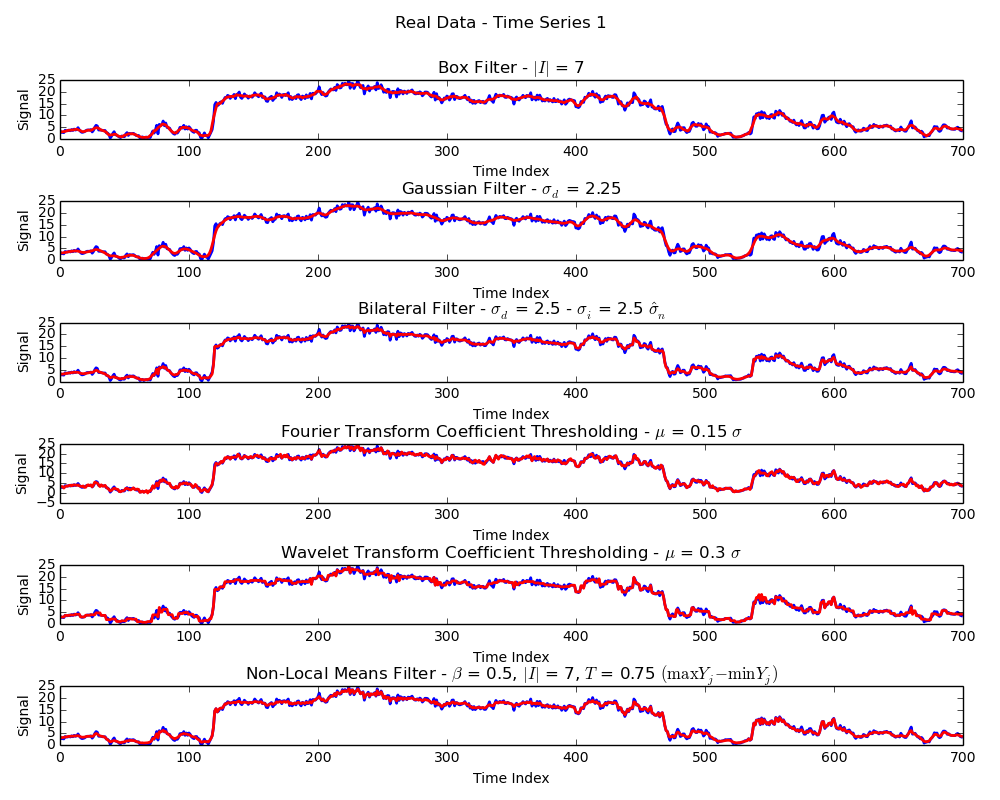
\includegraphics[width = 0.95 \textwidth]{TimeSeries1RealCompare.png}
\caption{Comparison on Real Data - Time Series 1}
\label{timeseries1realcompare}
\end{figure}

\begin{figure}[h!]
\centering
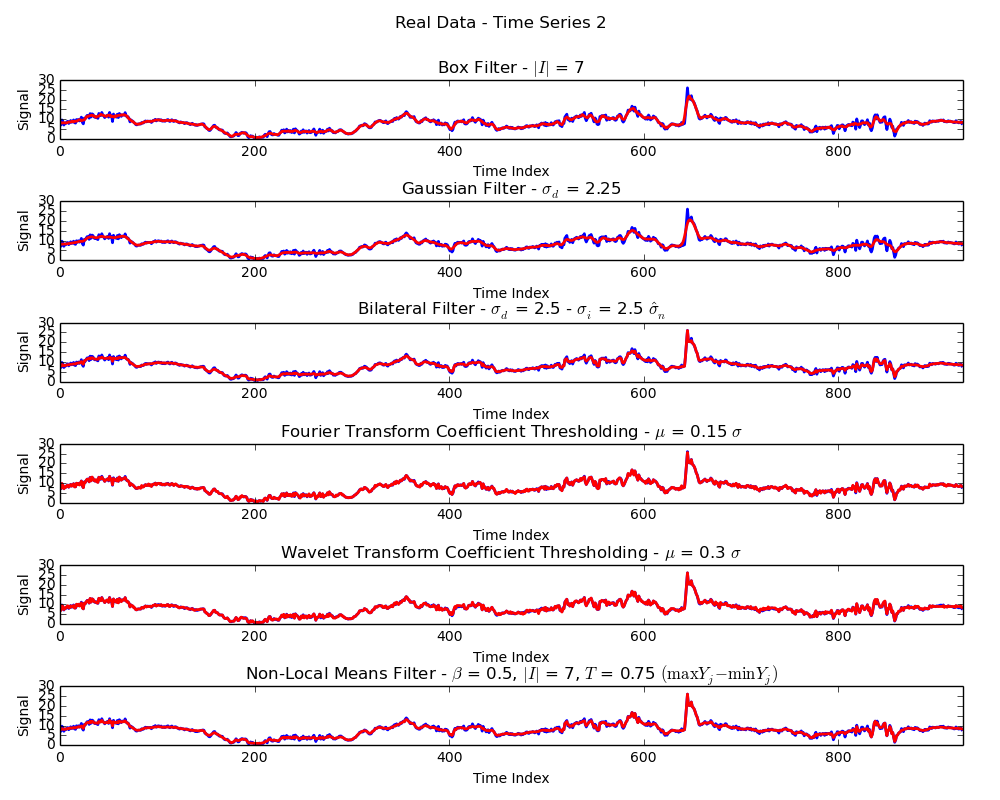
\includegraphics[width = 0.95 \textwidth]{TimeSeries2RealCompare.png}
\caption{Comparison on Real Data - Time Series 2}
\label{timeseries2realcompare}
\end{figure}

\begin{figure}[h!]
\centering
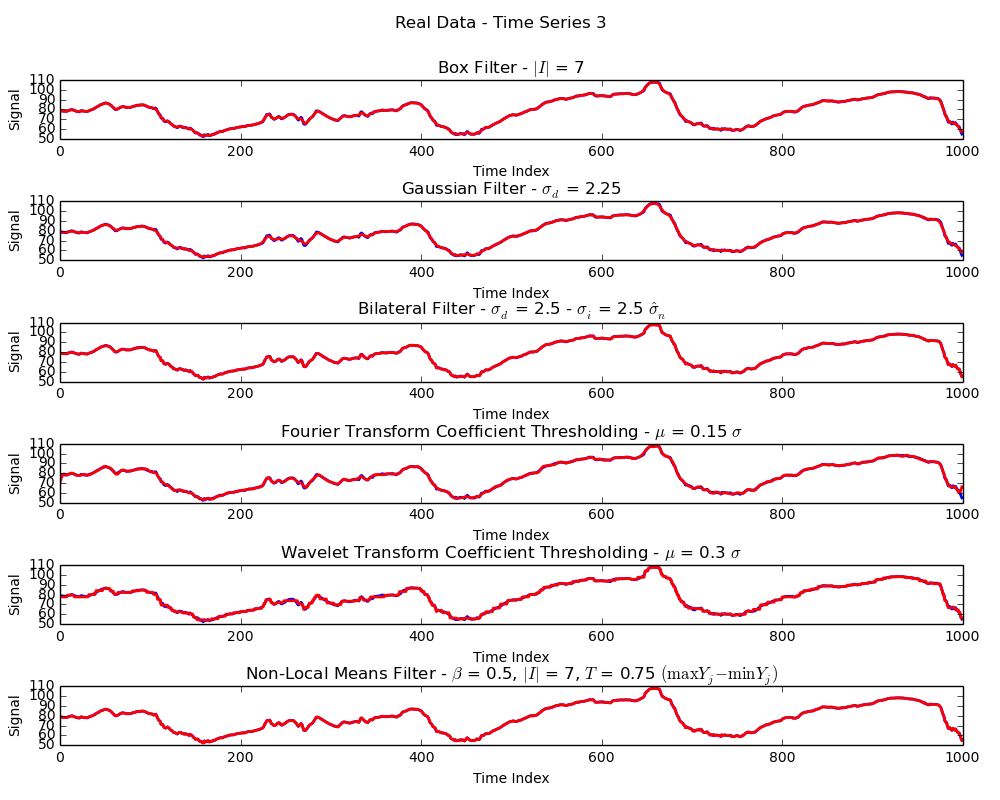
\includegraphics[width = 0.95 \textwidth]{TimeSeries3RealCompare.png}
\caption{Comparison on Real Data - Time Series 3}
\label{timeseries3realcompare}
\end{figure}


\section{Conclusions}

The box filter, Gaussian filter, Fourier transform coefficient thresholding, and wavelet transform coefficient thresholding consistently offer the worst performance, and all of these methods may in fact reduce PSNR for the time series. Also, Fourier transform coefficient thresholding is difficult to implement well for incremental time series. These techniques are not recommended as implemented. The wavelet transform can be improved with better choice of the family of wavelets.

Frequency based techniques such as Fourier transform coefficient thresholding or wavelet transform coefficient thresholding seem to do particularly poorly with a fixed parameter value. The more common practice with frequency techniques is to use SURE or another metric to fine tune the denoising parameters.

Non-Local Means offers a consistent improvement in PSNR, but its performance can be improved by paring it with a Bilateral filter. The parameter $\beta$ has an important impact on the performance of Non-Local Means. A future area of research should be to determine if some relationship between the variance of the time series and the estimated noise variance could be used to chose $\beta$. Also, Non-Local Means should theoretically perform better with longer time series, where more matching neighborhoods are possible. This possibility should be investigated. It is important to keep in mind that there is a tradeoff between keeping the data set small to ensure reasonable computation time and providing sufficient data to ensure good performance for Non-Local Means.

One or two iterations of the same Bilateral filter appears to offer the best consistent performance. Both have relatively stable optimal parameter settings, with a single iteration of the Bilateral filter being slightly more stable. Other versions of multiple iterations of a Bilateral filter offer less consistent results.


\FloatBarrier

%\bibliographystyle{acm}
\bibliographystyle{plain}
\bibliography{notes}

\end{document}
